\documentclass[UTF8]{ctexart}
\usepackage{subfigure}
\usepackage{caption}
\usepackage{amsmath,bm}
\usepackage{amssymb}
\usepackage{pifont}
\usepackage{geometry}
\usepackage{graphicx}
\usepackage{gensymb}
\usepackage{wrapfig}
\usepackage{titlesec}
\usepackage{float}
\usepackage{diagbox}
\usepackage{fancyhdr}
\usepackage{color}
\usepackage{bm}
\pagestyle{plain}
\geometry{a4paper,scale=0.8}
\CTEXsetup[format+={\raggedright}]{section} 
\title{通网2017-2018期末}
\author{Deschain}
\titlespacing*{\section}
{0pt}{0pt}{0pt}
\titlespacing*{\subsection}
{0pt}{0pt}{0pt}
\titlespacing*{\paragraph}
{0pt}{0pt}{0pt}
\titlespacing*{\subparagraph}
{0pt}{0pt}{0pt}
\titleformat*{\section}{\normalsize}
\begin{document}
\maketitle
\section*{一、问答题}
1.量化可以将连续随机变量离散化,量化过程中会产生量化噪声,量化噪声的来源可分为哪几种?如何降低
量化噪声?请解释在实际语音量化系统中,为什么采用非均匀量化?\\
2.时分多址与时分复用有什么区别?时分复用和频分复用有什么区别,各有什么优缺点?\\
3.某网络的拓扑结构如下所示。\\
(1)如果使用链路状态路由算法,当网络的路由搜索过程已经稳定后,写出网络稳定后的节点A,节点G的路由
表;\\
(2)如果使用距离矢量路由算法,当网络的路由搜索过程已经稳定后,写出网络稳定后的节点H,节点F的路由
表;\\
\begin{figure}[H]
  \centering
  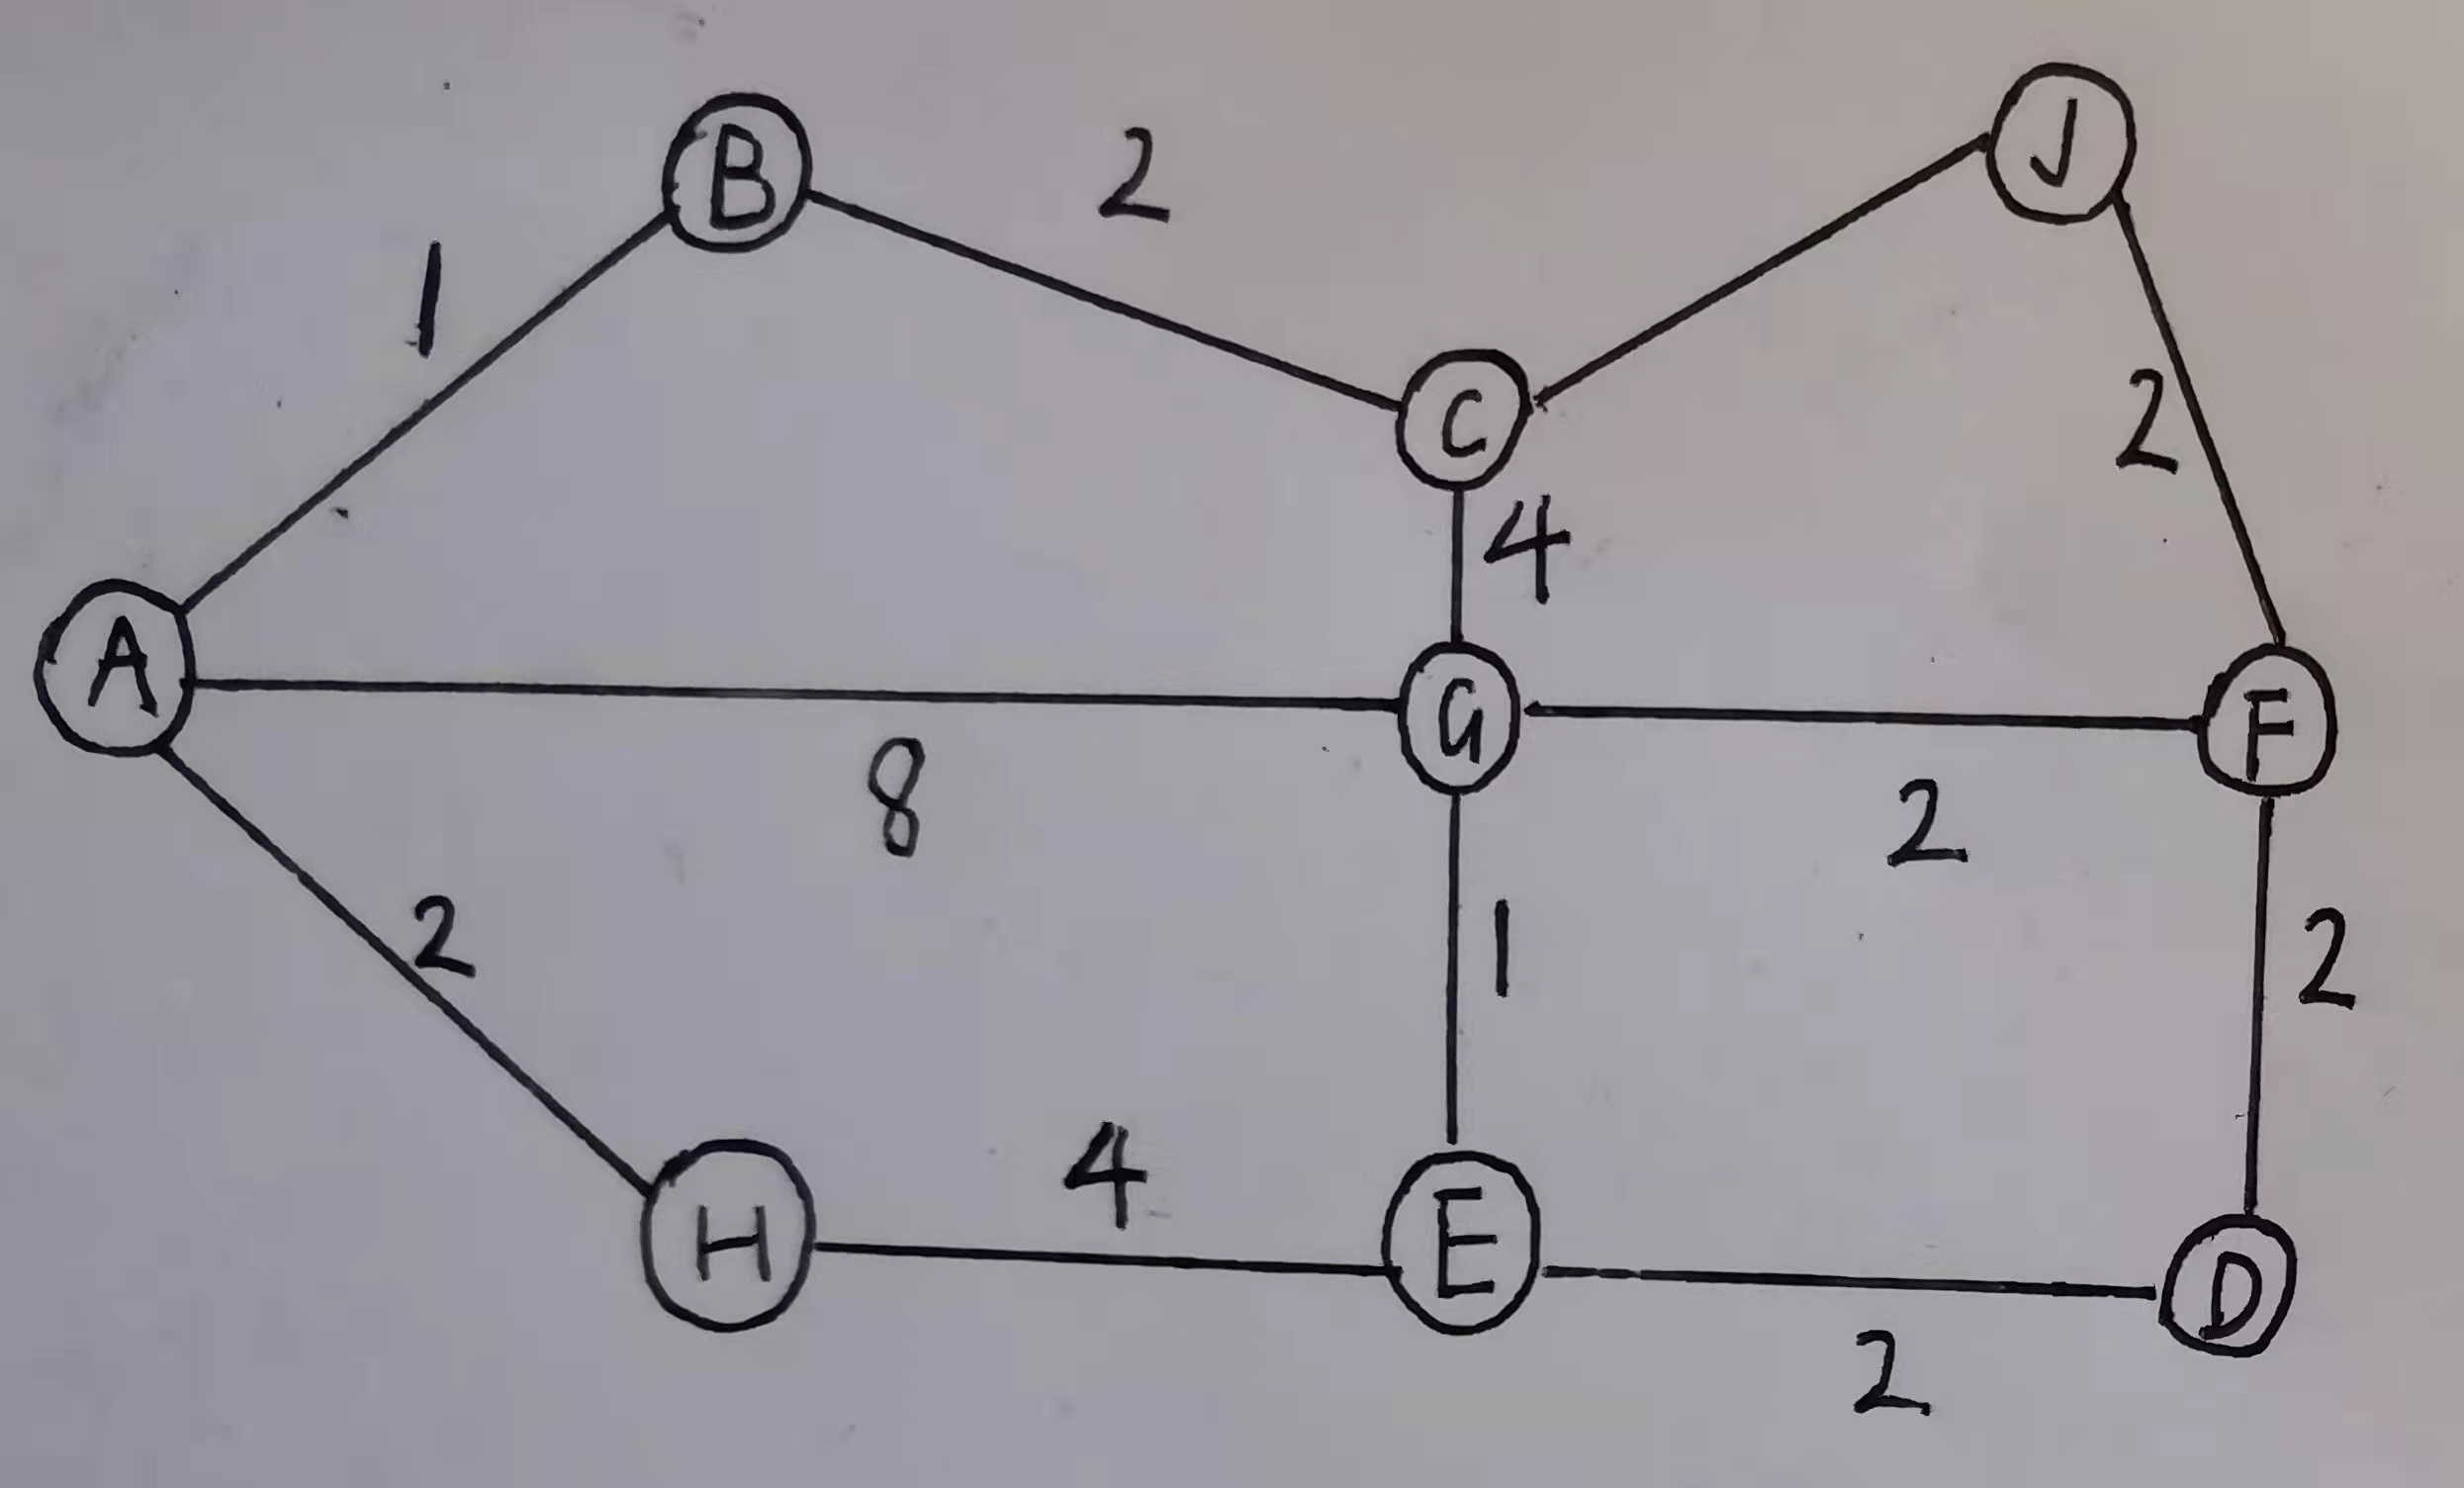
\includegraphics[width=6cm,height=4cm]{1_3.jpg}
\end{figure}
\section*{二、计算题}
1.某带限信道,仅允许频率范围在$\lvert f\rvert\leq0.1MHz$的信号无失真通过。接收机在无信号输入
时,在上述频率范围内测得的加性白高斯噪声的功率为$0.1\mu W$。为利用此信道传输10路PCM语音信号,
拟采用无信道编码的多电平基带传输方案,并使用根号升余弦滤波器,以0.08mW的平均功率进行传输。\\
问:\\
(1)设计基带传输方案,给出系统发送和接收框图、滚降系数、电平(符号)数、bit映射方法;\\
(2)根据你设计的参数,给出成形滤波器数学表达式,画出其幅频响应曲线,计算发送信号的功率谱并画图,
标明关键频率值。\\
(3)计算此基带传输系统的误比特率。\\
2.某通信系统,对需要传输比特流进行特定的编码和符号映射,具体方法为:\\
将3个待传信息比特$\bm{d}=(d_1,d_2,d_3)$进行编码形成4个二元符号$\bm{b}=(b_1,b_2,b_3,b_4)$,
规则为$b_i=d_i,(i<4),b_4=d_1\oplus d_2\oplus d_3$。\\
再对$\bm{b}$进行如下编码,形成另外4个二元符号,规则为:$\bm{c}=(c_1,c_2,c_3,c_4)$,其中$c_i
  =b_1\oplus\cdots\oplus b_i,(i\leq 4)$。\\
第$i$个符号的复数星座点为$I_i+jQ_i$,映射关系为:
\begin{equation*}
  \begin{aligned}
     & I_i=\begin{cases}
      1,\quad b_i=0  \\
      -1,\quad b_i=1 \\
    \end{cases},\quad\quad
    Q_i=\begin{cases}
      1,\quad c_i=0  \\
      -1,\quad c_i=1 \\
    \end{cases}
  \end{aligned}
\end{equation*}
问:\\
(1)从$\bm{d}$映射到$[\bm{b},\bm{c}]$,构成一种分组码,这种分组码的效率是多少?说明它是否为
线性分组码,为什么?\\
(2)写出这种码的生成矩阵,求最小汉明距离,它能纠几位错。\\
(3)写出所有可能的发送星座(复电平)序列(许用码字),求它们的最小欧氏距离。\\
(4)考虑噪声的影响,收到以下采样序列:$0.5-0.8j,-1.2-0.4j,0.8+1.5j,-0.3+0.7j$,写出你认为最
有可能的发送比特序列$\bm{d}$,要求介绍判定方法及过程。\\
3.在如图1所示的信道中,输入端输入为0或1,输出端输出为0或$e$或1,输入和输出之间的概率转移矩阵为
\begin{equation*}
  \begin{aligned}
     & \begin{bmatrix}
      p(0\lvert0) & p(e\lvert0) & p(1\lvert0) \\
      p(0\lvert1) & p(e\lvert1) & p(1\lvert1) \\
    \end{bmatrix}=
    \begin{bmatrix}
      1-\epsilon & \epsilon & 0          \\
      0          & \epsilon & 1-\epsilon \\
    \end{bmatrix}
  \end{aligned}
\end{equation*}
在如图2所示的系统中,有两个由图1描述的信道$H_1,H_2$,两个信道相互独立且转移矩阵相同(均为以上
矩阵),$X_1,X_2$为信道的输入符号,$Y_1,Y_2$表示经过信道后输出的符号。定义向信道容量为$C,X_1,
  X_2$独立等概分布,互信息量$R^{(1)}=I(\bm{X},\bm{Y})$,互信息量$R^{(2)}=I_1(X_1,\bm{Y})$。
\\问:\\
(1)当$\epsilon=0.2$时,计算$C$。\\
(2)当$\epsilon=0.2$,计算:$R^{(1)},R^{(2)}$。\\
(3)证明:在任意$\epsilon$下,$R^{(1)}=2C$。\\
(4)证明:在任意$\epsilon$下,不等关系$R^{(1)}-R^{(2)}\geq C\geq R^{(2)}$成立。\\
\begin{figure}[H]
  \centering
  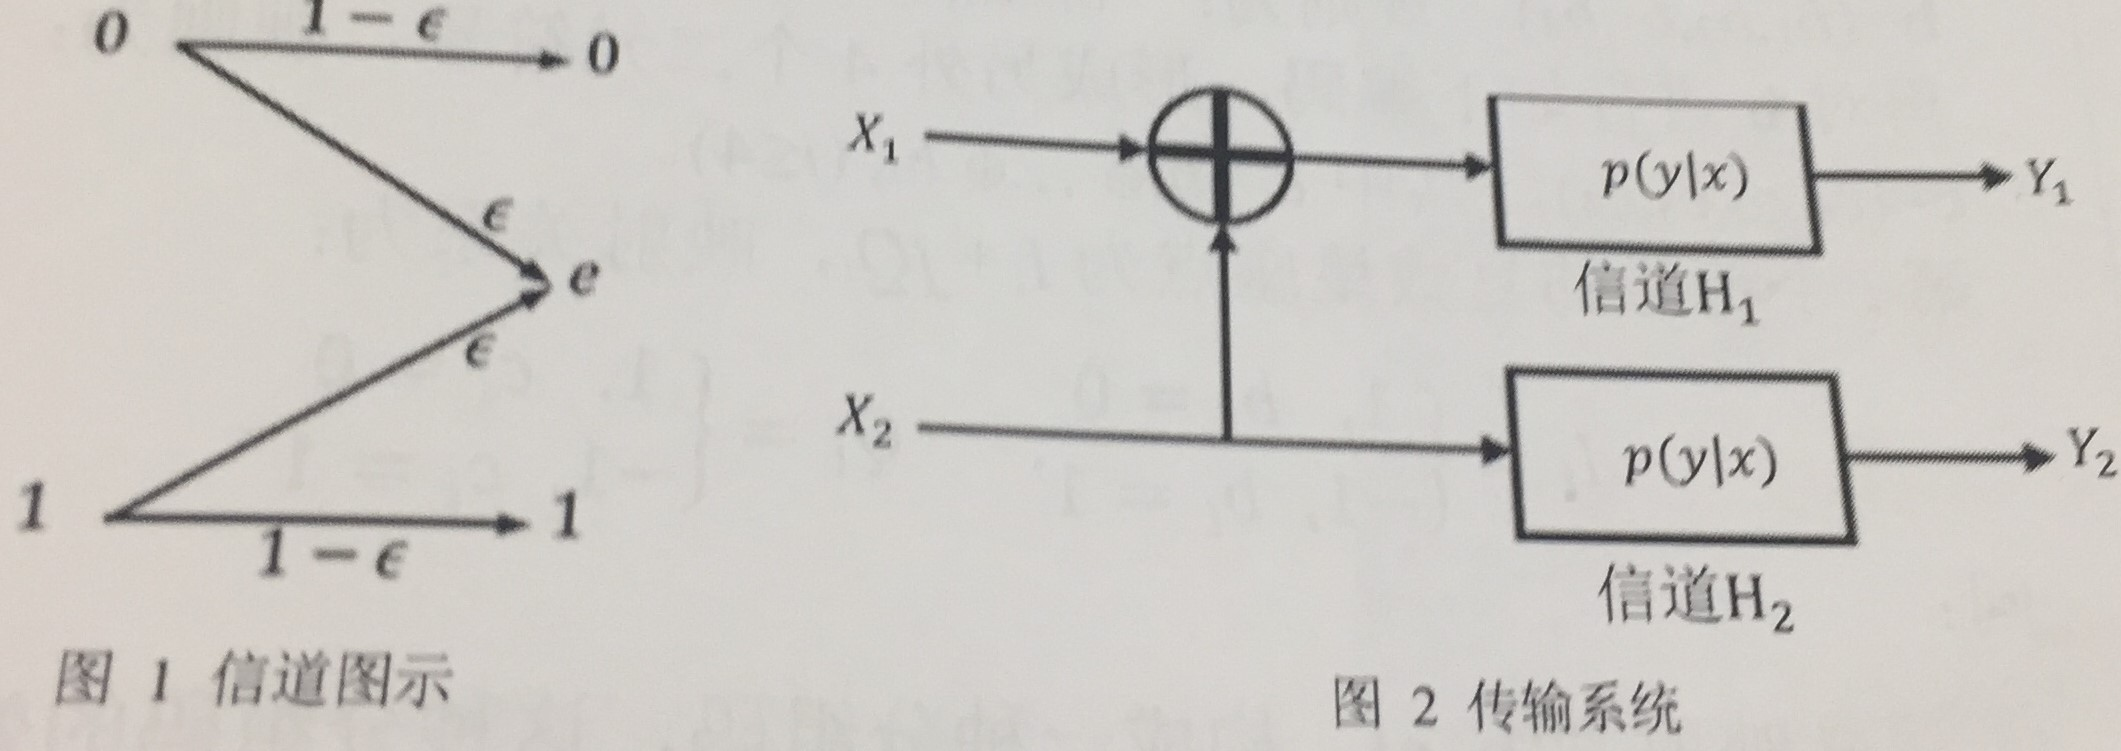
\includegraphics[width=10cm,height=4cm]{2_3.jpg}
\end{figure}
\end{document}